\documentclass[11pt,a4paper]{article}
\usepackage{amsmath,amssymb,amsthm}
\usepackage{booktabs}
\usepackage{array}
\usepackage{enumitem}
\usepackage{geometry}
\usepackage{graphicx}
\usepackage{xcolor}
\usepackage{tcolorbox}
\usepackage{listings}
\usepackage{tikz}
\usetikzlibrary{arrows.meta,positioning,calc,shapes.geometric,fit}
\usepackage[pdfencoding=auto,psdextra]{hyperref}

\geometry{margin=2.35cm}
\hypersetup{colorlinks=true,linkcolor=blue!55!black,citecolor=green!45!black,urlcolor=blue!60!black}

\newcommand{\E}{\mathbb{E}}
\newcommand{\R}{\mathbb{R}}
\newcommand{\N}{\mathcal{N}}
\newcommand{\norm}[1]{\left\lVert #1\right\rVert}
\newcommand{\inner}[2]{\left\langle #1,#2\right\rangle}
\newcommand{\sg}{\operatorname{sg}}
\newcommand{\logit}{\operatorname{logit}}
\newcommand{\RMS}{\operatorname{RMS}}
\newcommand{\old}{\mathrm{old}}
\newcommand{\data}{\mathrm{data}}

\theoremstyle{plain}
\newtheorem{theorem}{Theorem}[section]
\newtheorem{proposition}[theorem]{Proposition}
\newtheorem{corollary}[theorem]{Corollary}
\theoremstyle{definition}
\newtheorem{definition}[theorem]{Definition}
\newtheorem{remark}[theorem]{Remark}

\definecolor{codeblue}{RGB}{32,80,150}
\definecolor{codegreen}{RGB}{30,125,70}
\definecolor{codegray}{RGB}{100,100,100}
\definecolor{codepurple}{RGB}{125,45,145}
\definecolor{oldblue}{RGB}{48,105,180}
\definecolor{teacherred}{RGB}{190,65,55}
\definecolor{studentgreen}{RGB}{45,135,90}
\definecolor{riskorange}{RGB}{205,125,35}

\lstdefinestyle{python}{
  language=Python,
  basicstyle=\ttfamily\small,
  keywordstyle=\color{codeblue}\bfseries,
  commentstyle=\color{codegreen},
  stringstyle=\color{codepurple},
  numbers=left,
  numberstyle=\tiny\color{codegray},
  numbersep=7pt,
  breaklines=true,
  columns=fullflexible,
  keepspaces=true,
  showstringspaces=false,
  frame=single,
  framesep=5pt,
  xleftmargin=8pt,
  framexleftmargin=6pt
}
\lstdefinestyle{badpython}{
  style=python,
  backgroundcolor=\color{red!3},
  rulecolor=\color{red!45!black}
}
\lstdefinestyle{goodpython}{
  style=python,
  backgroundcolor=\color{green!3},
  rulecolor=\color{green!45!black}
}

\tikzset{
  flowbox/.style={
    draw,rounded corners=2pt,align=center,minimum height=10mm,
    minimum width=26mm,inner sep=5pt,font=\small
  },
  oldbox/.style={flowbox,draw=oldblue,fill=oldblue!7},
  teacherbox/.style={flowbox,draw=teacherred,fill=teacherred!7},
  studentbox/.style={flowbox,draw=studentgreen,fill=studentgreen!7},
  riskbox/.style={flowbox,draw=riskorange,fill=riskorange!8},
  neutralbox/.style={flowbox,draw=black!55,fill=black!3},
  flowarrow/.style={-{Latex[length=2.5mm]},thick,draw=black!70},
  oldline/.style={draw=oldblue,very thick},
  teacherline/.style={draw=teacherred,very thick},
  studentline/.style={draw=studentgreen,very thick},
  panel/.style={draw=black!25,rounded corners=3pt,fill=black!1,inner sep=7pt}
}

\title{\textbf{Arm A2: Forward-Risk P-OPD}\\[0.35em]
\large A first-principles tutorial on supervised evidence, Bayes calibration, and trust projection}
\author{Jayce-Ping}
\date{2026-08-03}

\begin{document}
\maketitle

\begin{abstract}
Arm A2 is a proposed ODE-compatible distillation rule.  An old student first produces a behavior
endpoint.  That endpoint is then re-noised along an independent forward flow-matching bridge, on
which a frozen teacher and frozen old student compete to predict the sampled velocity label.
Their squared-error difference becomes a detached sigmoid gate, while a separate metric
projection bounds the teacher displacement used as a regression target.

This tutorial derives the gate from a shared-covariance predictive-residual model, proves the
conditional risk decomposition and local replay gradient, and makes the event-sum, event-mean,
temperature, resolution, and trust-radius scales explicit.  It also distinguishes the exact
auxiliary likelihood from practical calibration, A2 from transition-mixture P-OPD (A3), and
forward-probe training from the ODE solver that generated the behavior endpoint.
\end{abstract}

\begin{tcolorbox}[colback=yellow!6,colframe=yellow!55!black,title=Status boundary]
\textbf{Arm A2 is a theory proposal, not a claim about an existing implementation.}
The existing target mode named \texttt{xopd\_target\_mode: p\_opd} denotes \textbf{Arm A3},
the stochastic transition-mixture construction.  Arm A4 is implemented under
\texttt{xopd\_target\_mode: marginal\_cfm}; the existing \texttt{direct} mode is only A0-like and
is not an exact implementation label for the A0/A1 taxonomy used here.  Nothing in this tutorial
asserts that an A2 API, configuration field, helper, trainer branch, or logging key already exists.
\end{tcolorbox}

\tableofcontents
\newpage

\section{The probability object comes first}
\label{sec:objects}

Fix a condition $C=c$.  Every distribution and expectation below is conditional on $C$, even
when $C$ is suppressed to keep notation readable.  A2 uses three layers, and only one of them
supplies its evidence:
\begin{enumerate}[leftmargin=1.6em]
\item an ODE \emph{behavior law} produces $x_{\data}$;
\item a forward FM \emph{supervised coupling} produces $(z,u)$;
\item an auxiliary \emph{predictive-residual likelihood} interprets the gate.
\end{enumerate}
It does not compare state densities and does not mix ODE marginals or stochastic transitions.

\begin{figure}[htbp]
\centering
\resizebox{0.96\textwidth}{!}{
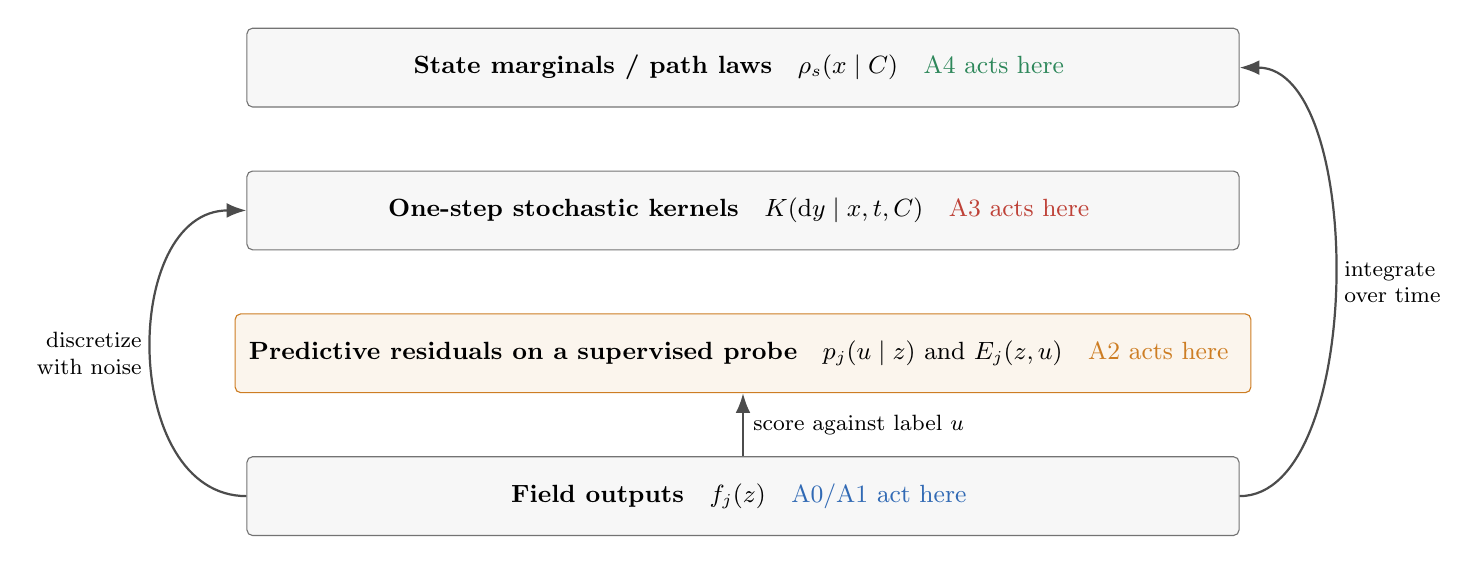
\begin{tikzpicture}[node distance=8mm]
  \node[neutralbox,minimum width=126mm] (marginal) {
    \textbf{State marginals / path laws}\quad $\rho_s(x\mid C)$\quad
    \textcolor{studentgreen}{A4 acts here}
  };
  \node[neutralbox,minimum width=126mm,below=of marginal] (kernel) {
    \textbf{One-step stochastic kernels}\quad $K(\mathrm d y\mid x,t,C)$\quad
    \textcolor{teacherred}{A3 acts here}
  };
  \node[riskbox,minimum width=126mm,below=of kernel] (risk) {
    \textbf{Predictive residuals on a supervised probe}\quad
    $p_j(u\mid z)$ and $E_j(z,u)$\quad \textcolor{riskorange}{A2 acts here}
  };
  \node[neutralbox,minimum width=126mm,below=of risk] (field) {
    \textbf{Field outputs}\quad $f_j(z)$\quad
    \textcolor{oldblue}{A0/A1 act here}
  };
  \draw[flowarrow] (field) -- node[right,font=\footnotesize] {score against label $u$} (risk);
  \draw[flowarrow] (field.west) .. controls +(-16mm,0) and +(-16mm,0) ..
    node[left,font=\footnotesize,align=right] {discretize\\with noise} (kernel.west);
  \draw[flowarrow] (field.east) .. controls +(16mm,0) and +(16mm,0) ..
    node[right,font=\footnotesize,align=left] {integrate\\over time} (marginal.east);
\end{tikzpicture}
}
\caption{Probability-object layers.  A2 evaluates predictive risk on a sampled FM label.  Moving
its formulas to the transition or marginal layer changes the method.}
\label{fig:object-layers}
\end{figure}

\begin{tcolorbox}[colback=blue!4,colframe=blue!50!black,title=One-sentence definition]
A2 asks whether the frozen teacher predicts a fresh forward-flow target better than the frozen old
student on an old-generated endpoint, then moves a detached regression target toward the teacher
by a separately trust-bounded amount.
\end{tcolorbox}

\section{From behavior rollout to a forward FM probe}
\label{sec:probe}

\subsection{Behavior endpoint}

Let the old student define the ODE used for behavior generation.  In a noise-to-data time
coordinate $t$,
\begin{equation}
\frac{\mathrm d X_t}{\mathrm d t}=v_{\old}(X_t,t,C),
\qquad X_0\sim\rho_{\mathrm{base}}(\cdot\mid C),
\qquad x_{\data}:=X_1^{\old}.
\label{eq:behavior-ode}
\end{equation}
The ODE solver may use any numerical grid appropriate to the model.  Once it returns
$x_{\data}$, A2 discards the solver path for the purpose of constructing its supervised probe.

\subsection{Fresh forward coupling}

Independently draw
\begin{equation}
s\sim\omega_{\mathrm{FM}}\ \text{on }[0,1],
\qquad
\varepsilon\sim\N(0,I_D),
\label{eq:fresh-draws}
\end{equation}
and define
\begin{equation}
x_s=(1-s)x_{\data}+s\varepsilon=x_{\data}+su,
\qquad
u=\varepsilon-x_{\data},
\qquad
z=(x_s,s,C).
\label{eq:forward-path}
\end{equation}
This bridge has \emph{data-to-noise} orientation: $s=0$ is the old-generated endpoint and $s=1$
is fresh Gaussian noise.  Its derivative is exactly $\partial_s x_s=u$.  A generation scheduler
may run in the opposite direction; the distinction is a coordinate/sign convention, not a reason
to reuse rollout timesteps.  The fresh $s$ and $\varepsilon$ decouple the training probe from the
ODE solver steps.  This is the standard linear conditional flow-matching coupling
\cite{flowmatching}, specialized to old-generated endpoints as formalized in the internal
five-arm note~\cite{internal-five-arm}.

\begin{figure}[htbp]
\centering
\resizebox{\textwidth}{!}{
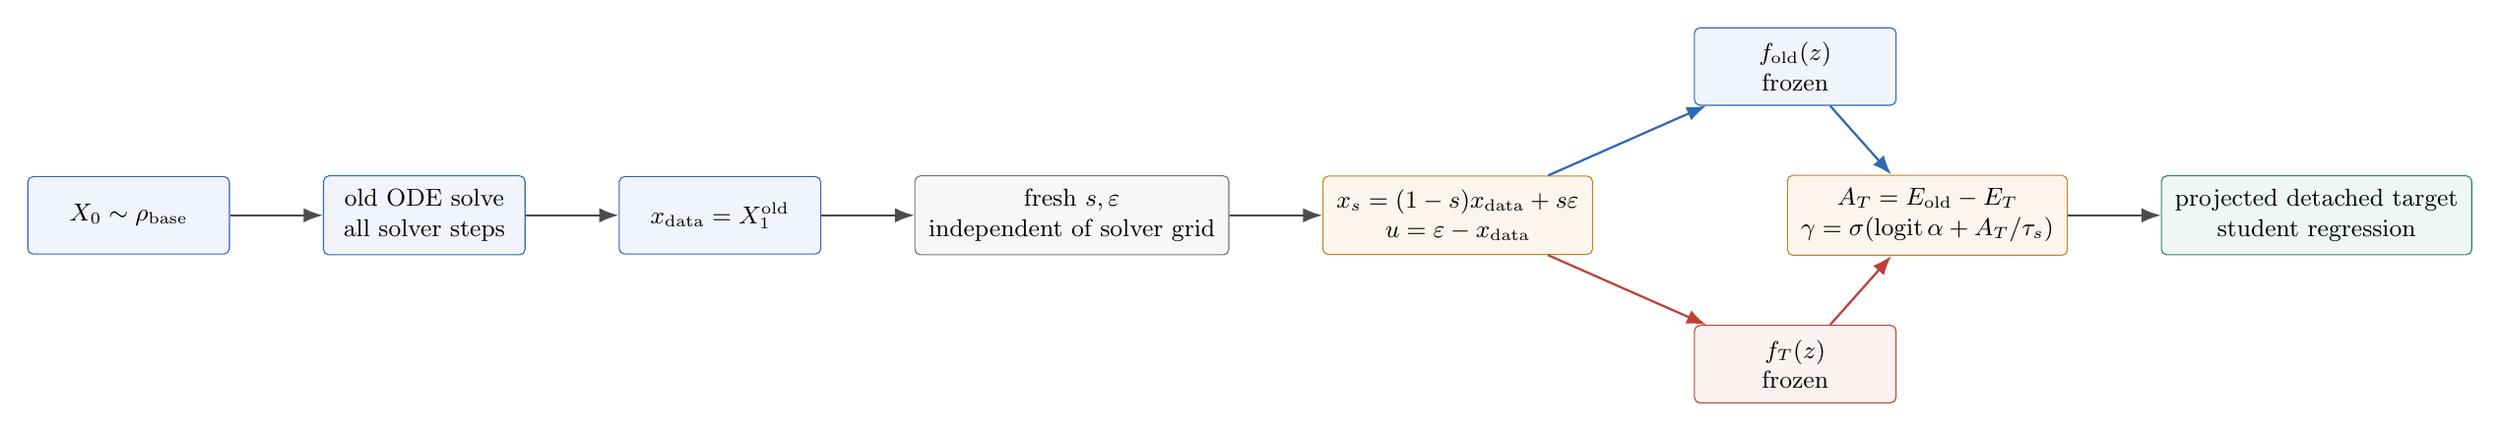
\begin{tikzpicture}[node distance=9mm and 12mm]
  \node[oldbox] (noise) {$X_0\sim\rho_{\mathrm{base}}$};
  \node[oldbox,right=of noise] (roll) {old ODE solve\\all solver steps};
  \node[oldbox,right=of roll] (endpoint) {$x_{\data}=X_1^{\old}$};
  \node[neutralbox,right=of endpoint] (fresh) {fresh $s,\varepsilon$\\independent of solver grid};
  \node[riskbox,right=of fresh] (probe) {$x_s=(1-s)x_{\data}+s\varepsilon$\\$u=\varepsilon-x_{\data}$};
  \node[oldbox,above right=9mm and 13mm of probe] (oldpred) {$f_{\old}(z)$\\frozen};
  \node[teacherbox,below right=9mm and 13mm of probe] (tpred) {$f_T(z)$\\frozen};
  \node[riskbox,right=25mm of probe] (gate) {$A_T=E_{\old}-E_T$\\$\gamma=\sigma(\logit\alpha+A_T/\tau_s)$};
  \node[studentbox,right=of gate] (target) {projected detached target\\student regression};
  \draw[flowarrow] (noise)--(roll);
  \draw[flowarrow] (roll)--(endpoint);
  \draw[flowarrow] (endpoint)--(fresh);
  \draw[flowarrow] (fresh)--(probe);
  \draw[flowarrow,draw=oldblue] (probe)--(oldpred);
  \draw[flowarrow,draw=teacherred] (probe)--(tpred);
  \draw[flowarrow,draw=oldblue] (oldpred)--(gate);
  \draw[flowarrow,draw=teacherred] (tpred)--(gate);
  \draw[flowarrow] (gate)--(target);
\end{tikzpicture}
}
\caption{Full A2 pipeline.  The behavior ODE supplies only the endpoint.  The FM probe uses fresh
randomness, and gradients belong only to the final student evaluation.}
\label{fig:a2-pipeline}
\end{figure}

\begin{lstlisting}[style=goodpython,caption={Good conceptual probe construction; names are illustrative, not APIs.}]
# A conceptual A2 iteration.
x_data = solve_old_behavior_ode(initial_noise, condition).detach()
s = sample_fm_time(batch_size)
epsilon = sample_standard_normal_like(x_data)

x_s = (1.0 - s) * x_data + s * epsilon
u = epsilon - x_data

with frozen_evaluation():
    f_old = old_model(x_s, s, condition)
    f_teacher = teacher_model(x_s, s, condition)
\end{lstlisting}

\begin{lstlisting}[style=badpython,caption={Bad: coupling the probe to stored ODE steps changes the evidence distribution.}]
# WRONG for A2: rollout states and solver labels are not the fresh FM probe.
for rollout_state, solver_time, solver_velocity in stored_old_trajectory:
    x_s = rollout_state
    s = solver_time
    u = solver_velocity
    compare_old_and_teacher(x_s, s, u)
\end{lstlisting}

\section{Residual energies and the gate}
\label{sec:gate}

Evaluate the frozen old and teacher predictors on the same $z$; both predict the native
data-to-noise target $u$.  Let $D$ be the number of non-batch event coordinates and define
\begin{equation}
E_j(z,u)=\frac{1}{2c_D}\norm{u-f_j(z)}_2^2,
\qquad
c_D=
\begin{cases}
1,&\text{event sum},\\
D,&\text{event mean}.
\end{cases}
\label{eq:energies}
\end{equation}
The teacher advantage and gate are
\begin{equation}
A_T=E_{\old}-E_T,
\qquad
\gamma_T=\sigma\!\left(\logit\alpha+\frac{A_T}{\tau_s}\right),
\qquad 0<\alpha<1,\quad \tau_s>0.
\label{eq:gate}
\end{equation}
Thus $A_T>0$ means the teacher is closer to the sampled target than the old student.  At
$A_T=0$, the gate is the prior $\alpha$.

\begin{figure}[htbp]
\centering
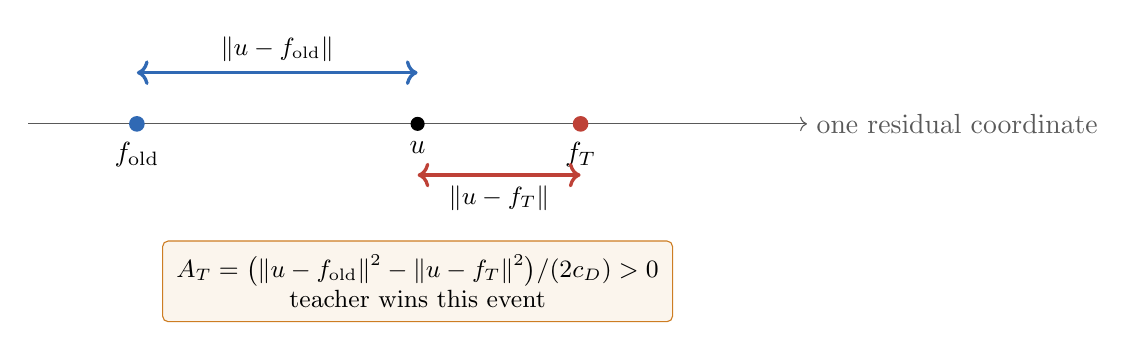
\begin{tikzpicture}[x=1.15cm,y=1.0cm]
  \draw[->,black!65] (-4.3,0)--(4.3,0) node[right] {one residual coordinate};
  \node[circle,fill=black,inner sep=1.8pt,label=below:$u$] (u) at (0,0) {};
  \node[circle,fill=oldblue,inner sep=2pt,label=below:$f_{\old}$] (o) at (-3.1,0) {};
  \node[circle,fill=teacherred,inner sep=2pt,label=below:$f_T$] (t) at (1.8,0) {};
  \draw[oldline,<->] (-3.1,0.65)--(0,0.65)
    node[midway,above,font=\small] {$\norm{u-f_{\old}}$};
  \draw[teacherline,<->] (0,-0.65)--(1.8,-0.65)
    node[midway,below,font=\small] {$\norm{u-f_T}$};
  \node[riskbox,minimum width=62mm] at (0,-2.0)
    {$A_T=\bigl(\norm{u-f_{\old}}^2-\norm{u-f_T}^2\bigr)/(2c_D)>0$\\teacher wins this event};
\end{tikzpicture}
\caption{Residual-energy geometry in one coordinate.  In $D$ dimensions, squared Euclidean
distances replace the intervals; the sign convention remains the same.}
\label{fig:residual-geometry}
\end{figure}

\section{The exact auxiliary Gaussian interpretation}
\label{sec:bayes}

\begin{proposition}[Exact posterior under shared predictive covariance]
\label{prop:posterior}
Fix $z$, assume $\sigma_r^2(s)>0$, and introduce $B\in\{\old,T\}$ with
$\Pr(B=T)=\alpha$.  Declare
\begin{equation}
p_j(u\mid z)
=(2\pi\sigma_r^2(s))^{-D/2}
\exp\!\left[-\frac{\norm{u-f_j(z)}^2}{2\sigma_r^2(s)}\right].
\label{eq:predictive-model}
\end{equation}
Then
\begin{equation}
\Pr(B=T\mid u,z)
=\sigma\!\left(\logit\alpha+\frac{c_DA_T}{\sigma_r^2(s)}\right).
\label{eq:posterior}
\end{equation}
Consequently, the gate in \eqref{eq:gate} is this exact posterior when
\begin{equation}
\boxed{\tau_s=\frac{\sigma_r^2(s)}{c_D}}.
\label{eq:exact-temperature}
\end{equation}
Whenever $A_T$ is nonzero on the relevant support, equality of the two logits there also requires
this temperature.
\end{proposition}

\begin{proof}
Shared covariance makes the Gaussian normalizers cancel:
\begin{align}
\log\frac{p_T(u\mid z)}{p_{\old}(u\mid z)}
&=\frac{\norm{u-f_{\old}}^2-\norm{u-f_T}^2}{2\sigma_r^2(s)}
=\frac{c_DA_T}{\sigma_r^2(s)}.
\end{align}
Posterior odds equal prior odds times the likelihood ratio.  Taking logits gives
\eqref{eq:posterior}; comparison with \eqref{eq:gate} gives \eqref{eq:exact-temperature}.
\end{proof}

\begin{figure}[htbp]
\centering
\resizebox{0.94\textwidth}{!}{
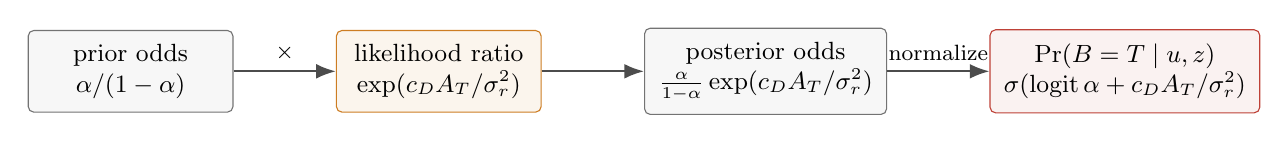
\begin{tikzpicture}[node distance=9mm and 13mm]
  \node[neutralbox] (prior) {prior odds\\$\alpha/(1-\alpha)$};
  \node[riskbox,right=of prior] (lr) {likelihood ratio\\
    $\exp(c_DA_T/\sigma_r^2)$};
  \node[neutralbox,right=of lr] (odds) {posterior odds\\
    $\frac{\alpha}{1-\alpha}\exp(c_DA_T/\sigma_r^2)$};
  \node[teacherbox,right=of odds] (post) {$\Pr(B=T\mid u,z)$\\
    $\sigma(\logit\alpha+c_DA_T/\sigma_r^2)$};
  \draw[flowarrow] (prior)--node[above,font=\footnotesize] {$\times$} (lr);
  \draw[flowarrow] (lr)--(odds);
  \draw[flowarrow] (odds)--node[above,font=\footnotesize] {normalize} (post);
\end{tikzpicture}
}
\caption{Bayes posterior and logit.  The sign is positive because a lower teacher energy makes
$A_T=E_{\old}-E_T$ positive.}
\label{fig:bayes-logit}
\end{figure}

\paragraph{Declared residual covariance is not forward corruption noise.}
The covariance $\sigma_r^2(s)I_D$ in \eqref{eq:predictive-model} models uncertainty of the
\emph{predictive label residual} $u-f_j(z)$ after conditioning on $z$.  The fresh
$\varepsilon\sim\N(0,I_D)$ in \eqref{eq:fresh-draws} creates the forward coupling and determines
$x_s$.  These are different random objects.  There is no automatic identity such as
$\sigma_r^2(s)=s^2$ or $\sigma_r^2(s)=1$.  Unequal old and teacher covariances would introduce
log-determinant and unequal quadratic terms, so a plain energy difference would no longer be the
exact posterior logit.

\begin{tcolorbox}[colback=yellow!5,colframe=yellow!50!black,title=Exact likelihood versus calibrated surrogate]
With event-sum energies and $\tau_s=\sigma_r^2(s)$, the gate is exact for the declared joint
$D$-dimensional likelihood.  With event-mean energies, exactness requires
$\tau_s=\sigma_r^2(s)/D$.  Choosing a resolution-stable numerical temperature, centering $A_T$,
normalizing by a running scale, or clipping logits may be useful, but then the gate is a
\emph{calibrated surrogate}, not that exact joint-likelihood posterior.
\end{tcolorbox}

\section{What one sampled advantage estimates}
\label{sec:risk}

Define the conditional mean and irreducible variance under old-generated endpoints and fresh
forward noise:
\begin{equation}
m_{\old}(z)=\E[u\mid z],
\qquad
V_{\old}(z)=\E[\norm{u-m_{\old}(z)}^2\mid z].
\label{eq:conditional-moments}
\end{equation}

\begin{proposition}[Conditional risk decomposition and cancellation]
\label{prop:risk}
For either frozen predictor $j\in\{\old,T\}$,
\begin{equation}
\E[E_j\mid z]
=\frac{1}{2c_D}
\left(V_{\old}(z)+\norm{f_j(z)-m_{\old}(z)}^2\right),
\label{eq:risk-decomposition}
\end{equation}
and therefore
\begin{equation}
\E[A_T\mid z]
=\frac{\norm{f_{\old}-m_{\old}}^2-\norm{f_T-m_{\old}}^2}{2c_D}.
\label{eq:mean-advantage}
\end{equation}
Thus $A_T$ is a one-sample unbiased estimator of the conditional risk difference.
\end{proposition}

\begin{proof}
Write $u-f_j=(u-m_{\old})+(m_{\old}-f_j)$ and expand.  The conditional cross term vanishes because
$\E[u-m_{\old}\mid z]=0$.  Subtracting the old and teacher expressions cancels the same
irreducible variance $V_{\old}$.
\end{proof}

\begin{figure}[htbp]
\centering
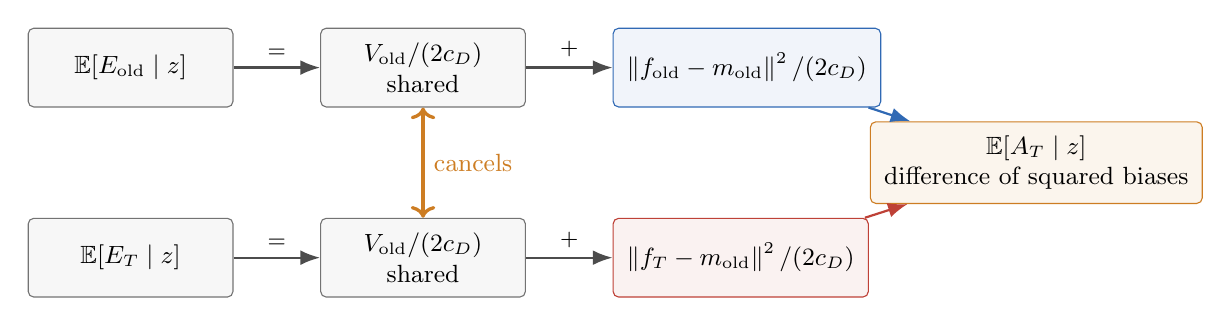
\begin{tikzpicture}[node distance=7mm and 11mm]
  \node[neutralbox] (ol) {$\E[E_{\old}\mid z]$};
  \node[neutralbox,right=of ol] (ov) {$V_{\old}/(2c_D)$\\shared};
  \node[oldbox,right=of ov] (ob) {$\norm{f_{\old}-m_{\old}}^2/(2c_D)$};
  \draw[flowarrow] (ol)--node[above,font=\footnotesize] {$=$} (ov);
  \draw[flowarrow] (ov)--node[above,font=\footnotesize] {$+$} (ob);
  \node[neutralbox,below=14mm of ol] (tl) {$\E[E_T\mid z]$};
  \node[neutralbox,right=of tl] (tv) {$V_{\old}/(2c_D)$\\shared};
  \node[teacherbox,right=of tv] (tb) {$\norm{f_T-m_{\old}}^2/(2c_D)$};
  \draw[flowarrow] (tl)--node[above,font=\footnotesize] {$=$} (tv);
  \draw[flowarrow] (tv)--node[above,font=\footnotesize] {$+$} (tb);
  \draw[<->,very thick,riskorange] (ov.south)--node[right,font=\small] {cancels} (tv.north);
  \node[riskbox,right=16mm of $(ob)!0.5!(tb)$] (diff)
    {$\E[A_T\mid z]$\\difference of squared biases};
  \draw[flowarrow,draw=oldblue] (ob)--(diff);
  \draw[flowarrow,draw=teacherred] (tb)--(diff);
\end{tikzpicture}
\caption{Conditional risk decomposition.  A2 compares approximation biases after the shared
irreducible label variance cancels.}
\label{fig:risk-decomposition}
\end{figure}

\paragraph{Expectation and sigmoid do not commute.}
Although $A_T$ is an unbiased estimator of the conditional mean risk difference, its transformed
gate is generally not an unbiased estimator of the sigmoid of that mean:
\begin{equation}
\E[\gamma_T\mid z]\ne
\sigma\!\left(\logit\alpha+\frac{\E[A_T\mid z]}{\tau_s}\right)
\quad\text{in general}.
\label{eq:sigmoid-bias}
\end{equation}
The discrepancy depends on the full conditional distribution of $A_T$, not only its mean.

\begin{figure}[htbp]
\centering
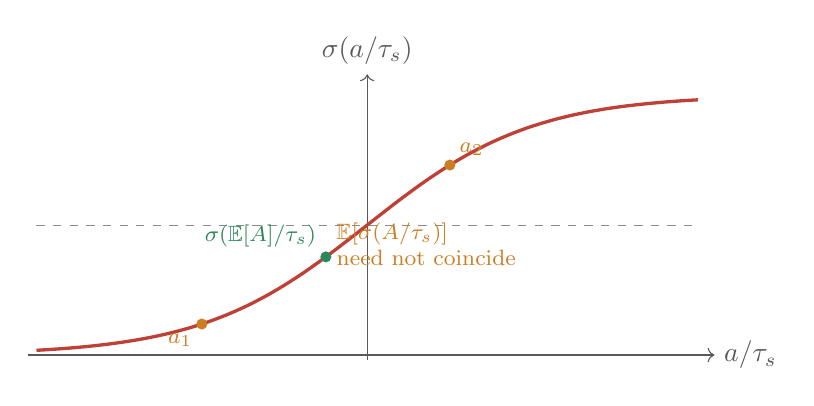
\begin{tikzpicture}[x=1.05cm,y=3.3cm]
  \draw[->,black!65] (-4.1,0)--(4.2,0) node[right] {$a/\tau_s$};
  \draw[->,black!65] (0,-0.02)--(0,1.08) node[above] {$\sigma(a/\tau_s)$};
  \draw[teacherline,smooth] plot[domain=-4:4,samples=80] (\x,{1/(1+exp(-\x))});
  \draw[dashed,black!45] (-4,0.5)--(4,0.5);
  \coordinate (a1) at (-2,{1/(1+exp(2))});
  \coordinate (a2) at (1,{1/(1+exp(-1))});
  \fill[riskorange] (a1) circle (2pt) node[below left,font=\footnotesize] {$a_1$};
  \fill[riskorange] (a2) circle (2pt) node[above right,font=\footnotesize] {$a_2$};
  \coordinate (mean) at (-0.5,{1/(1+exp(0.5))});
  \fill[studentgreen] (mean) circle (2pt)
    node[above left,font=\footnotesize,align=right] {$\sigma(\E[A]/\tau_s)$};
  \draw[very thick,riskorange] (-0.5,0.425)--(-0.5,0.425)
    node[right,font=\footnotesize,align=left] {$\E[\sigma(A/\tau_s)]$\\need not coincide};
\end{tikzpicture}
\caption{Noncommutation of expectation and sigmoid, schematically for a two-point advantage law.
Equality occurs only in special cases (for example, a degenerate advantage).}
\label{fig:sigmoid-bias}
\end{figure}

\paragraph{Why the old field need not be the conditional mean.}
$f_{\old}$ generated $x_{\data}$ through an ODE, but $m_{\old}(z)=\E[u\mid x_s,s,C]$ belongs to a
new coupling formed by re-noising the endpoint with fresh $\varepsilon$.  Generation competence
does not imply $f_{\old}(z)=m_{\old}(z)$ on that coupling.  A2 only compares $f_{\old}$ and $f_T$
under the old-endpoint probe distribution; it does not assume either is Bayes-optimal.

\section{Trust projection and the detached target}
\label{sec:trust}

Let $G_s$ be positive definite and define
$\norm{a}_{G_s}^2=a^\top G_sa$.  Let $r_s>0$ be a $G_s$-norm output radius; it is an
event-$L^2$ radius only when $G_s=I$.  Set
\begin{equation}
d=f_T-f_{\old},
\qquad
c=
\begin{cases}
1,&\norm d_{G_s}=0,\\
\min\{1,r_s/\norm d_{G_s}\},&\norm d_{G_s}>0.
\end{cases}
\label{eq:projection}
\end{equation}
The frozen, detached target and regression loss are
\begin{align}
f_\gamma(z,u)
&=f_{\old}(z)+\sg(\gamma_T)c\,d,
\label{eq:target}\\
\mathcal L_{\mathrm{A2}}(\theta)
&=\E\!\left[\frac{1}{2c_D}
\norm{f_\theta(z)-f_\gamma(z,u)}_{G_s}^2\right].
\label{eq:a2-loss}
\end{align}
The whole right-hand side of \eqref{eq:target} is a target: old and teacher predictions are frozen,
$c$ is computed from frozen values, and $\gamma_T$ is explicitly stop-gradient.

\begin{proposition}[Trust bound and exact-replay gradient]
\label{prop:gradient}
For every event,
\begin{equation}
\norm{f_\gamma-f_{\old}}_{G_s}\le r_s.
\label{eq:trust-bound}
\end{equation}
If $f_{\theta_{\old}}=f_{\old}$ exactly and
$J_{\old}=\left.\partial f_\theta/\partial\theta\right|_{\theta_{\old}}$, then
\begin{equation}
\left.\nabla_\theta\mathcal L_{\mathrm{A2}}\right|_{\theta_{\old}}
=-\frac{1}{c_D}\E\!\left[
\gamma_Tc\,J_{\old}^{\top}G_s(f_T-f_{\old})
\right].
\label{eq:local-gradient}
\end{equation}
\end{proposition}

\begin{proof}
Equation \eqref{eq:target} gives
$\norm{f_\gamma-f_{\old}}_{G_s}=\gamma_Tc\norm d_{G_s}
\le c\norm d_{G_s}\le r_s$.
Differentiating \eqref{eq:a2-loss} only through $f_\theta$ yields
$c_D^{-1}J_\theta^\top G_s(f_\theta-f_\gamma)$.  At replay,
$f_\theta-f_\gamma=-\gamma_Tcd$, proving the negative sign in
\eqref{eq:local-gradient}.  This is the aggregate regression gradient.  For a single event, its
self-Jacobian contribution is teacherward when the local Jacobian geometry permits; a shared
minibatch parameter update also contains cross-event interactions and therefore does not
guarantee pointwise teacherward movement for every sampled output.
\end{proof}

\begin{figure}[htbp]
\centering
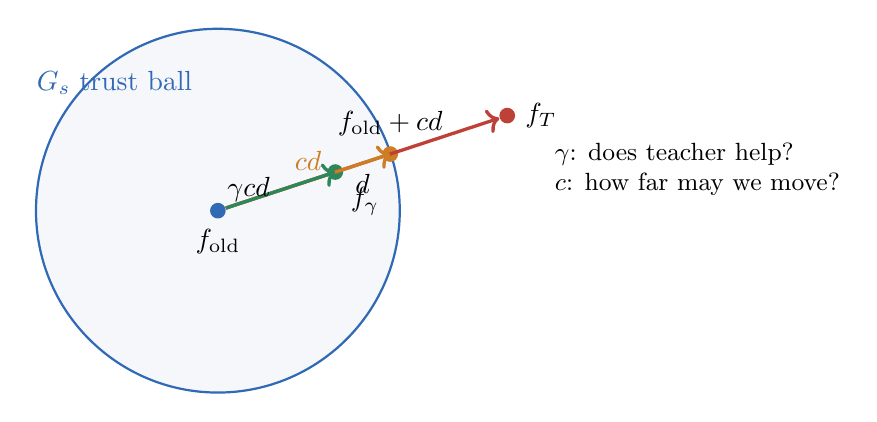
\begin{tikzpicture}[x=1.05cm,y=1.05cm]
  \draw[fill=oldblue!5,draw=oldblue,thick] (0,0) circle (2.2);
  \node[circle,fill=oldblue,inner sep=2pt,label=below:$f_{\old}$] (o) at (0,0) {};
  \node[circle,fill=teacherred,inner sep=2pt,label=right:$f_T$] (t) at (3.5,1.15) {};
  \coordinate (p) at (2.085,0.685);
  \node[circle,fill=riskorange,inner sep=2pt,label=above:$f_{\old}+cd$] at (p) {};
  \coordinate (g) at (1.42,0.467);
  \node[circle,fill=studentgreen,inner sep=2pt,label=below right:$f_\gamma$] at (g) {};
  \draw[teacherline,->] (o)--(t) node[midway,below] {$d$};
  \draw[riskorange,very thick,->] (o)--(p) node[midway,above] {$cd$};
  \draw[studentline,very thick,->] (o)--(g) node[midway,left] {$\gamma cd$};
  \node[text=oldblue] at (-1.25,1.55) {$G_s$ trust ball};
  \node[align=left,font=\small] at (5.8,0.5)
    {$\gamma$: does teacher help?\\$c$: how far may we move?};
\end{tikzpicture}
\caption{Trust-ball projection.  The projection coefficient bounds the full teacher displacement;
the gate can only shorten it further.}
\label{fig:trust-ball}
\end{figure}

\begin{lstlisting}[style=goodpython,caption={Good conceptual detached gate, projection, and student-only regression.}]
event_axes = tuple(range(1, u.ndim))
energy_old = (u - f_old).square().sum(dim=event_axes) / (2.0 * c_D)
energy_teacher = (
    (u - f_teacher).square().sum(dim=event_axes) / (2.0 * c_D)
)
advantage_teacher = energy_old - energy_teacher
gate = sigmoid(logit(alpha) + advantage_teacher / temperature_s)

displacement = f_teacher - f_old
displacement_norm = metric_norm(displacement, metric_s)
projection = where(
    displacement_norm == 0,
    ones_like(displacement_norm),
    minimum(ones_like(displacement_norm), radius_s / displacement_norm),
)
target = (
    f_old + gate.detach() * projection * displacement
).detach()

f_student = student_model(x_s, s, condition)
loss_per_sample = metric_square(
    f_student - target, metric_s
).sum(dim=event_axes) / (2.0 * c_D)
loss = loss_per_sample.mean()
\end{lstlisting}

\begin{lstlisting}[style=badpython,caption={Bad: gradient leakage makes the gate and target gameable.}]
# WRONG: teacher/old/gate are part of the autograd graph.
f_old = trainable_student(x_s, s, condition)
f_teacher = teacher_model(x_s, s, condition)
gate = sigmoid(logit(alpha) + (energy(f_old) - energy(f_teacher)) / tau)
target = f_old + gate * (f_teacher - f_old)
loss = squared_error(trainable_student(x_s, s, condition), target)
loss.backward()  # Optimizes through the evidence and target construction.
\end{lstlisting}

\paragraph{RMS radius.}
If $G_s=I$ and the desired per-coordinate radius is $r_s^{\RMS}$, then the corresponding event
radius is $r_s=\sqrt D\,r_s^{\RMS}$.  Mixing an RMS radius with an unnormalized event norm silently
tightens the trust region as resolution grows.

\section{Dimension, temperature, and saturation}
\label{sec:scaling}

For any $\delta\in(0,\tfrac12)$,
\begin{align}
\gamma_T\le\delta
&\iff A_T\le\tau_s\bigl(\logit\delta-\logit\alpha\bigr),
\label{eq:low-saturation}\\
\gamma_T\ge1-\delta
&\iff A_T\ge\tau_s\bigl(\logit(1-\delta)-\logit\alpha\bigr).
\label{eq:high-saturation}
\end{align}
At a fixed per-coordinate advantage $a$, event-sum evidence is approximately $A_T=Da$, whereas
event-mean evidence is $A_T=a$.  A fixed sum-gate temperature therefore becomes more binary as
$D$ grows.

\begin{figure}[htbp]
\centering
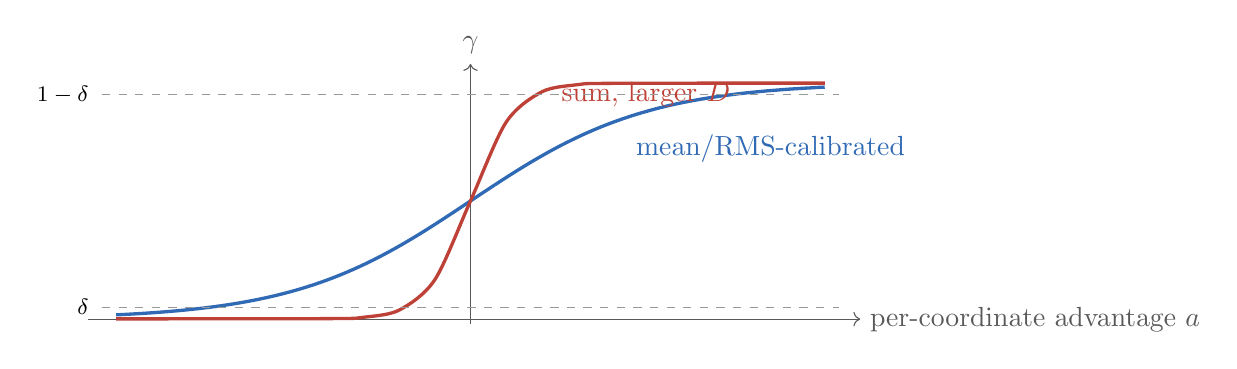
\begin{tikzpicture}[x=0.9cm,y=3.0cm]
  \draw[->,black!65] (-5.4,0)--(5.5,0) node[right] {per-coordinate advantage $a$};
  \draw[->,black!65] (0,-0.02)--(0,1.08) node[above] {$\gamma$};
  \draw[oldline,smooth] plot[domain=-5:5,samples=100] (\x,{1/(1+exp(-0.8*\x))});
  \draw[teacherline,smooth] plot coordinates {
    (-5,0.001) (-2,0.002) (-1.5,0.008) (-1,0.039) (-0.5,0.168)
    (0,0.5) (0.5,0.832) (1,0.961) (1.5,0.992) (2,0.998) (5,0.999)
  };
  \node[text=oldblue,anchor=west] at (2.2,0.72) {mean/RMS-calibrated};
  \node[text=teacherred,anchor=west] at (1.15,0.95) {sum, larger $D$};
  \draw[dashed,black!40] (-5.2,0.05)--(5.2,0.05);
  \draw[dashed,black!40] (-5.2,0.95)--(5.2,0.95);
  \node[font=\footnotesize,anchor=east] at (-5.25,0.05) {$\delta$};
  \node[font=\footnotesize,anchor=east] at (-5.25,0.95) {$1-\delta$};
\end{tikzpicture}
\caption{Event-sum versus event-mean saturation.  The curves illustrate identical per-coordinate
risk gaps with different effective logits; exact slopes depend on $D/\tau_s$.}
\label{fig:sum-mean}
\end{figure}

\subsection{Resolution transfer rules}

\begin{enumerate}[leftmargin=1.6em]
\item \textbf{Exact joint-likelihood convention.}  Use event sums and
      $\tau_s=\sigma_r^2(s)$.  If resolution changes, the log likelihood legitimately accumulates
      more coordinate evidence and the posterior may sharpen.
\item \textbf{Equivalent exact mean parameterization.}  Divide energies by $D$ and also divide
      temperature by $D$: $\tau_s=\sigma_r^2(s)/D$.  The logit is unchanged.
\item \textbf{Practical resolution-stable surrogate.}  Use event means and keep a numerical
      temperature on the per-coordinate scale.  This deliberately changes the implied
      predictive covariance and must be labeled as calibration.
\item \textbf{Trust scale.}  Transfer $r_s^{\RMS}$, not a fixed event-$L^2$ radius, when $D$
      changes.
\end{enumerate}

\begin{lstlisting}[style=goodpython,caption={Good conceptual calibration diagnostics retain both event scales.}]
advantage_sum = energy_old_sum - energy_teacher_sum
advantage_per_dimension = advantage_sum / event_dimension

log_scalar("advantage_sum", advantage_sum)
log_scalar("advantage_per_dimension", advantage_per_dimension)
log_quantiles("gate", gate, probabilities=(0.01, 0.1, 0.5, 0.9, 0.99))
log_scalar("gate_entropy", binary_entropy(gate))
log_scalar("gate_low_saturation", mean(gate <= saturation_delta))
log_scalar("gate_high_saturation", mean(gate >= 1 - saturation_delta))
\end{lstlisting}

\section{One inner step and stale behavior data}
\label{sec:stale}

The cleanest A2 interpretation freezes an old model, collects behavior endpoints, constructs
targets, and performs \emph{one} inner optimizer step before refreshing the old snapshot and its
data.  At exact replay, Proposition~\ref{prop:gradient} gives the intended local direction.

Several inner steps on the same batch are not mathematically forbidden, but after the first step
$f_\theta\ne f_{\old}$ while $x_{\data}$, $f_{\old}$, $f_T$, $\gamma_T$, $c$, and $f_\gamma$
remain stale.  Optimization then fits a fixed supervised target rather than repeatedly
re-evaluating whether the teacher helps under the current behavior distribution.  Large replay
counts can move parameters far from the local trust interpretation even though every individual
output target remains within radius $r_s$ of the frozen old output.  Output-space target trust is
not a parameter-space or rollout-distribution trust guarantee.

\begin{tcolorbox}[colback=yellow!5,colframe=yellow!50!black,title=Recommended semantic unit]
Treat ``freeze old $\rightarrow$ roll out $\rightarrow$ draw fresh probes $\rightarrow$ build
detached targets $\rightarrow$ take one inner step $\rightarrow$ refresh'' as the reference A2
unit.  If replay is introduced for efficiency, ablate the replay count and measure realized
post-update output displacement and endpoint drift.
\end{tcolorbox}

\section{A0--A4 and neighboring forward-probe methods}
\label{sec:comparisons}

\begin{figure}[htbp]
\centering
\resizebox{\textwidth}{!}{
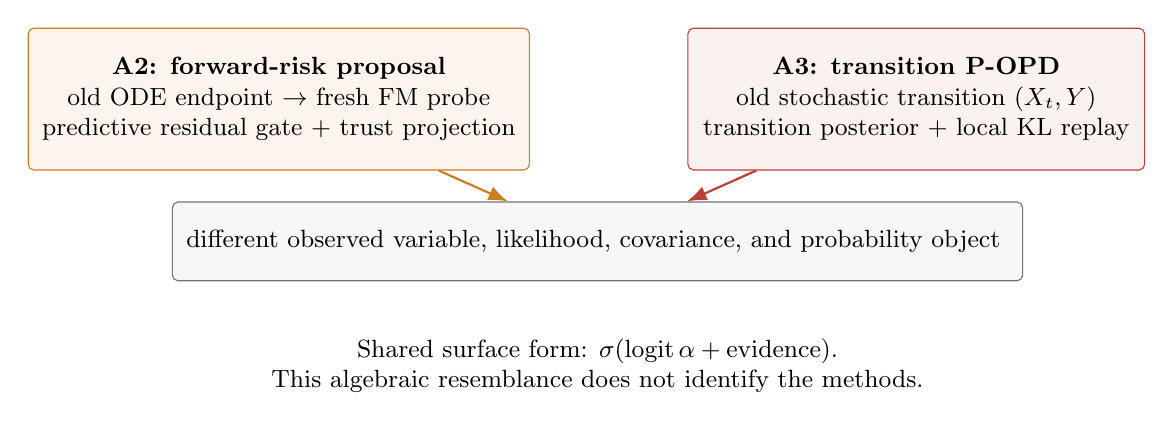
\begin{tikzpicture}[node distance=7mm and 12mm]
  \node[riskbox,minimum width=58mm,minimum height=18mm] (a2) {
    \textbf{A2: forward-risk proposal}\\old ODE endpoint $\to$ fresh FM probe\\
    predictive residual gate + trust projection
  };
  \node[teacherbox,minimum width=58mm,minimum height=18mm,right=20mm of a2] (a3) {
    \textbf{A3: transition P-OPD}\\old stochastic transition $(X_t,Y)$\\
    transition posterior + local KL replay
  };
  \node[neutralbox,below=13mm of $(a2)!0.5!(a3)$] (different) {
    different observed variable, likelihood, covariance, and probability object
  };
  \draw[flowarrow,draw=riskorange] (a2)--(different);
  \draw[flowarrow,draw=teacherred] (a3)--(different);
  \node[font=\small,align=center,below=6mm of different] {
    Shared surface form: $\sigma(\logit\alpha+\text{evidence})$.\\
    This algebraic resemblance does not identify the methods.
  };
\end{tikzpicture}
}
\caption{A2 versus A3.  The configured \texttt{p\_opd} path is A3; A2 remains a distinct theory
proposal based on fresh supervised forward-flow evidence.}
\label{fig:a2-vs-a3}
\end{figure}

\begin{center}
\small
\begin{tabular}{@{}
  >{\raggedright\arraybackslash}p{0.09\textwidth}
  >{\raggedright\arraybackslash}p{0.23\textwidth}
  >{\raggedright\arraybackslash}p{0.29\textwidth}
  >{\raggedright\arraybackslash}p{0.30\textwidth}@{}}
\toprule
arm & evidence distribution & target operation & mathematical status\\
\midrule
A0 & old-generated states & direct teacher regression & field matching under old occupancy\\
\addlinespace
A1 & old-generated states & fixed arithmetic interpolation or quadratic trust step &
field-space geometry; no sample-dependent predictive test\\
\addlinespace
\textbf{A2} & old ODE endpoints re-noised by fresh FM coupling & risk-gated, projected,
detached teacher displacement & proposed supervised predictive-risk rule\\
\addlinespace
A3 & old SDE transition and sampled next state & transition-posterior gate with local replay &
stochastic transition-mixture P-OPD; existing \texttt{p\_opd}\\
\addlinespace
A4 & old/teacher source trajectory branch & regress sampled source velocity &
implemented ODE time-marginal mixture through \texttt{marginal\_cfm}\\
\bottomrule
\end{tabular}
\end{center}

\paragraph{Relation to DPO, NFT, AWM, DGPO, and CRD.}
These decoupled methods share a useful mechanism: generate behavior outputs first, then sample
fresh forward corruption times/noise and train on single-step forward probes.  DPO uses
preference pairs; DiffusionNFT forms a reward-weighted contrast between implicit positive and
negative policies; AWM uses advantage-weighted matching; DGPO adds groupwise
preference/advantage structure; and Centered Reward Distillation (CRD) matches centered external
rewards to implicit rewards defined by forward prediction errors.  This family resemblance
motivates A2's solver-decoupled probe, but none of those objectives automatically supplies A2's
Bayes interpretation, old-versus-teacher risk gate, or trust projection.  Those must be derived
and validated separately.
The transition-posterior interpretation of A3 is related to DiffusionOPD and trust-region policy
distillation~\cite{diffusionopd,topd}, while the distinct A4 marginal construction is developed in
the internal A4 tutorial~\cite{internal-a4}.

\begin{tcolorbox}[colback=red!4,colframe=red!45!black,title=Terminology boundary]
A2 is \textbf{not} a state-density-ratio method, \textbf{not} a transition-mixture KL method, and
\textbf{not} a marginal-mixture method.  Its exact probabilistic statement is only the auxiliary
predictive likelihood $p_j(u\mid z)$ in Proposition~\ref{prop:posterior}.
\end{tcolorbox}

\section{Conceptual implementation blueprint}
\label{sec:blueprint}

The following is an algorithmic blueprint, not a map to existing symbols.
\begin{enumerate}[leftmargin=1.6em]
\item Freeze an old snapshot and a teacher.
\item Solve the old ODE and retain its endpoint $x_{\data}$.
\item Draw fresh $s$ and $\varepsilon$; construct $(x_s,u,z)$ using
      \eqref{eq:forward-path}.
\item In no-gradient evaluation, compute $f_{\old}(z)$ and $f_T(z)$ on the same input and in the
      same native target convention.
\item Compute $A_T$, a detached gate, and the metric projection using one declared sum/mean and
      temperature convention.
\item Detach $f_\gamma$ completely.
\item Run exactly one gradient-enabled student forward on $z$ and regress to $f_\gamma$.
\item After the update, measure displacement; refresh behavior data before interpreting another
      step as a fresh local A2 step.
\end{enumerate}

\begin{lstlisting}[style=goodpython,caption={Good high-level A2 blueprint with explicit invariant checks.}]
# Conceptual pseudocode only; these names do not claim repository APIs.
x_data = old_ode_endpoint(condition, initial_noise).detach()
s, epsilon = fresh_forward_probe_randomness(x_data)
x_s, u = make_linear_forward_probe(x_data, s, epsilon)

with frozen_evaluation():
    f_old = old_predictor(x_s, s, condition)
    f_teacher = teacher_predictor(x_s, s, condition)

if f_old.shape != u.shape or f_teacher.shape != u.shape:
    raise ValueError(
        "expected old, teacher, and target shapes to match; "
        f"old={f_old.shape}, teacher={f_teacher.shape}, target={u.shape}"
    )
if temperature_s <= 0:
    raise ValueError(
        f"expected positive A2 temperature, received {temperature_s!r}"
    )

gate, projection = detached_gate_and_projection(
    u=u,
    f_old=f_old,
    f_teacher=f_teacher,
    alpha=alpha,
    temperature_s=temperature_s,
    radius_s=radius_s,
    event_dimension=u[0].numel(),
)
target = (
    f_old + gate * projection * (f_teacher - f_old)
).detach()
f_student = student_predictor(x_s, s, condition)
student_forward_regression(f_student, target)
\end{lstlisting}

\begin{lstlisting}[style=badpython,caption={Bad: silent fallbacks erase the method's declared statistical meaning.}]
# WRONG: do not hide invalid scales or missing predictions.
try:
    f_teacher = teacher_predictor(x_s, s, condition)
except Exception:
    f_teacher = f_old

temperature_s = max(temperature_s, 1e-8)
event_dimension = guessed_dimension if shape_is_confusing else x_s.numel()
gate = sigmoid((energy_old - energy_teacher) / temperature_s)
\end{lstlisting}

The bad listing is doubly dangerous: it swallows teacher failures and silently changes scale
definitions.  An implementation should validate types, shapes, finiteness, ranges, and target
orientation before using them, then raise specific errors containing the received values and
relevant identifiers.

\section{Logging, calibration, and ablations}
\label{sec:logging}

\subsection{Minimum diagnostics}

Log distributions, not only means:
\begin{itemize}[leftmargin=1.5em]
\item a consistently computed \texttt{advantage\_sum} and
      $\texttt{advantage\_mean}=\texttt{advantage\_sum}/D$, including timestep-conditioned
      quantiles, plus an explicit record of which normalization drives the gate;
\item $\gamma_T$ quantiles, binary entropy
      $-\gamma\log\gamma-(1-\gamma)\log(1-\gamma)$, and low/high saturation rates;
\item teacher-win rate $\Pr(A_T>0)$;
\item $\norm d_{\RMS}=\norm d_2/\sqrt D$, $\norm d_2$, and projection coefficient $c$;
\item forward regression loss binned by $s$;
\item realized post-update displacement
      $\norm{f_{\theta^+}(z)-f_{\old}(z)}_{\RMS}$ and its ratio to the intended target movement;
\item total and, where possible, componentwise gradient norms and clipping rates.
\end{itemize}
Gate statistics diagnose \emph{whether} evidence selects the teacher; $d$ and $c$ diagnose
\emph{how large} the proposed movement is; realized displacement and gradient norms diagnose
whether optimization actually executes that proposal.

\subsection{Ablation matrix}

\begin{center}
\small
\begin{tabular}{@{}
  >{\raggedright\arraybackslash}p{0.22\textwidth}
  >{\raggedright\arraybackslash}p{0.26\textwidth}
  >{\raggedright\arraybackslash}p{0.22\textwidth}
  >{\raggedright\arraybackslash}p{0.21\textwidth}@{}}
\toprule
axis & levels & hold fixed & decisive readout\\
\midrule
energy normalization & sum; mean & same samples/models & separately labeled
$A_T^{\mathrm{sum}}$ and $A_T^{\mathrm{mean}}$, saturation versus $D$\\
\addlinespace
temperature & exact $\sigma_r^2/c_D$; calibrated constant; $s$-schedule &
normalization and prior & gate calibration, entropy, teacher-win-conditioned loss\\
\addlinespace
prior $\alpha$ & low; $0.5$; high & temperature & gate quantiles and update magnitude\\
\addlinespace
trust radius & no clipping; RMS grid; $G_s=I$ event-$L^2$ grid & gate & $c$, realized displacement,
stability\\
\addlinespace
gate & constant $\alpha$; hard win; sigmoid & same projected $d$ & quality, variance,
saturation sensitivity\\
\addlinespace
probe time law & uniform; stratified; endpoint-biased & corruption formula & forward loss and
mean-normalized advantage by $s$\\
\addlinespace
inner replay & 1; 2; 4+ steps per behavior batch & optimizer budget where feasible & stale-target
drift and endpoint shift\\
\addlinespace
resolution & matched low/high $D$ & per-coordinate corruption & transfer of entropy,
$r^{\RMS}$, quality\\
\bottomrule
\end{tabular}
\end{center}

For the exact-likelihood ablation, report the declared $\sigma_r^2(s)$ and verify
\eqref{eq:exact-temperature}.  For calibrated surrogates, report the calibration transform
explicitly and avoid posterior language unless empirical calibration is measured.

\section{Limitations and recommended implementation order}
\label{sec:limitations}

\subsection{Limitations}

\begin{enumerate}[leftmargin=1.6em]
\item \textbf{Proposal status.}  The derivation does not establish production correctness,
      distributed behavior, or gains on any model.
\item \textbf{Auxiliary model dependence.}  Bayes exactness holds only for the declared
      shared covariance residual model and matched temperature.
\item \textbf{One-sample gate variance.}  $A_T$ is unbiased for a risk difference, but expectation
      and sigmoid do not commute; the gate can also be noisy or saturated.
\item \textbf{Old occupancy.}  Evidence is gathered on endpoints produced by the old ODE; it says
      nothing directly about teacher-only regions.
\item \textbf{Conditional-mean mismatch.}  Neither frozen model need equal $\E[u\mid z]$.
\item \textbf{Local trust only.}  The output target is bounded at sampled probes, not globally in
      parameter space, endpoint distribution, or perceptual quality.
\item \textbf{Metric choice.}  $G_s$, $r_s$, and the native prediction parameterization determine
      the geometry and require model-specific validation.
\item \textbf{Staleness.}  Multi-step replay weakens the exact-replay local-gradient story.
\item \textbf{Compute.}  Every probe requires frozen old and teacher predictions plus a
      gradient-enabled student prediction.
\end{enumerate}

\subsection{Recommended order}

\begin{enumerate}[leftmargin=1.6em]
\item Build a CPU tensor-level reference for energies, posterior logits, projection, and the
      replay-gradient sign.
\item Verify prediction-target orientation and event axes on one real model batch.
\item Add diagnostic-only forward probes with no optimizer update; measure separately labeled
      sum- and mean-normalized advantages, gate saturation, $d$ scales, and timestep dependence.
\item Choose either exact joint-likelihood scaling or an explicitly named calibrated surrogate.
\item Add detached targets and one inner step with a conservative RMS trust radius.
\item Measure realized displacement, gradients, and endpoint drift before increasing replay or
      radius.
\item Run the normalization, temperature, radius, and resolution ablations in
      Section~\ref{sec:logging}.
\item Only after single-device numerical validation, design distributed call order, snapshot
      lifecycle, checkpointing, and production configuration.
\end{enumerate}

\section{Summary}

Arm A2 separates three questions:
\[
\boxed{
\begin{gathered}
\text{Where is evidence measured?}\quad
x_{\data}\xrightarrow[\varepsilon,s\ \mathrm{fresh}]{\text{forward FM}}(z,u),\\
\text{Does the teacher help?}\quad
A_T=E_{\old}-E_T,\quad
\gamma_T=\sigma(\logit\alpha+A_T/\tau_s),\\
\text{How far may the target move?}\quad
c=\min(1,r_s/\norm d_{G_s}),\quad
f_\gamma=f_{\old}+\sg(\gamma_T)cd.
\end{gathered}}
\]
The shared-covariance posterior is obtained with
$\tau_s=\sigma_r^2(s)/c_D$, and this scale is identifiable wherever the advantage is nonzero.
The risk advantage is one-sample unbiased because irreducible conditional variance cancels, but
expectation and sigmoid generally do not commute.  The detached target yields the negative
replay-gradient sign in \eqref{eq:local-gradient}; its single-event self-Jacobian contribution is
teacherward when the local geometry permits, without a pointwise minibatch guarantee.  These
statements define a forward-risk proposal; they do not turn A2 into A3, A4, or an existing target
mode.

\begin{thebibliography}{9}

\bibitem{flowmatching}
Yaron Lipman, Ricky T. Q. Chen, Heli Ben-Hamu, Maximilian Nickel, and Matt Le.
\newblock Flow Matching for Generative Modeling.
\newblock \emph{International Conference on Learning Representations}, 2023.
\newblock \url{https://arxiv.org/abs/2210.02747}.

\bibitem{diffusionopd}
Quanhao Li, Junqiu Yu, Kaixun Jiang, et al.
\newblock DiffusionOPD: A Unified Perspective of On-Policy Distillation in Diffusion Models.
\newblock 2026.
\newblock \url{https://arxiv.org/abs/2605.15055}.

\bibitem{topd}
Zhengpeng Xie, Li Lyna Zhang, Zeke Xie, and Mao Yang.
\newblock Trust Region Policy Distillation.
\newblock 2026.
\newblock \url{https://arxiv.org/abs/2607.04751}.

\bibitem{internal-five-arm}
Jayce-Ping.
\newblock Generalized P-OPD: Five-Arm Formalization.
\newblock Internal Flow-Factory note
\href{run:../arms/generalized_popd_five_arm_formalization.pdf}
{(linked PDF)}, 2026.

\bibitem{internal-saturation}
Jayce-Ping.
\newblock P-OPD Exact-Sum Gate Saturation.
\newblock Internal Flow-Factory note
\href{run:../p_opd/popd_exact_sum_gate_saturation.pdf}
{(linked PDF)}, 2026.

\bibitem{internal-a4}
Jayce-Ping.
\newblock Arm A4: Mixture-of-Density.
\newblock Internal Flow-Factory tutorial
\href{run:../marginal_cfm/arm_a4_marginal_mixture_cfm_tutorial.pdf}
{(linked PDF)}, 2026.

\end{thebibliography}

\end{document}
